\section{Additional Details on the Proposed \nameDataset Dataset.}

The \texttt{\nameDataset} dataset is built using high-quality, commercially licensed 3D environments that include both realistic indoor and outdoor scenes. For each environment, we populate the space with multiple animated human characters. 
The character assets are sourced from Mixamo \cite{mixamo} and HUMOTO \cite{Lu_2025_HUMOTO}, and each character is manually textured and refined to ensure realistic geometry, appearance, and material quality. 
The animations span a diverse range of human motions, including locomotion, gestures, and human-object interactions.
Examples of scenes are shown in \cref{fig:visualexample}. 
Please refer to the complementary website for the video examples.

To capture rich spatial coverage, we generate four distinct camera trajectories for every scene. Camera paths include rotational orbits, linear tracking motions, and smoothly curved arcs. A dedicated validity module ensures that each trajectory:
(1) begins at a collision-free location with clear visibility of the main character,
(2) maintains non-intersecting movement with the environment throughout the path, and
(3) preserves full subject visibility across all viewpoints.

Each trajectory is rendered into a 120-frame sequence at a resolution of $1080 \times 1080$ pixels, providing dense temporal sampling with high visual fidelity. This yields three multi-view video sequences per scene, each covering the full motion duration with consistent lighting, textures, and geometry. Overall, we rendered 1500 videos from 500 animations, each with 120 videos full grid rendering, leading to 180k videos.

For temporal-control training, we could sample any time variants from these sequences, including slow motion, reverse playback, bullet-time around arbitrary frames, and non-monotonic time patterns such as forward–backward oscillation. These augmented temporal signals are illustrated in \cref{fig:sampling}.

\begin{figure}[ht]
    \centering
    \vspace{-3mm}
    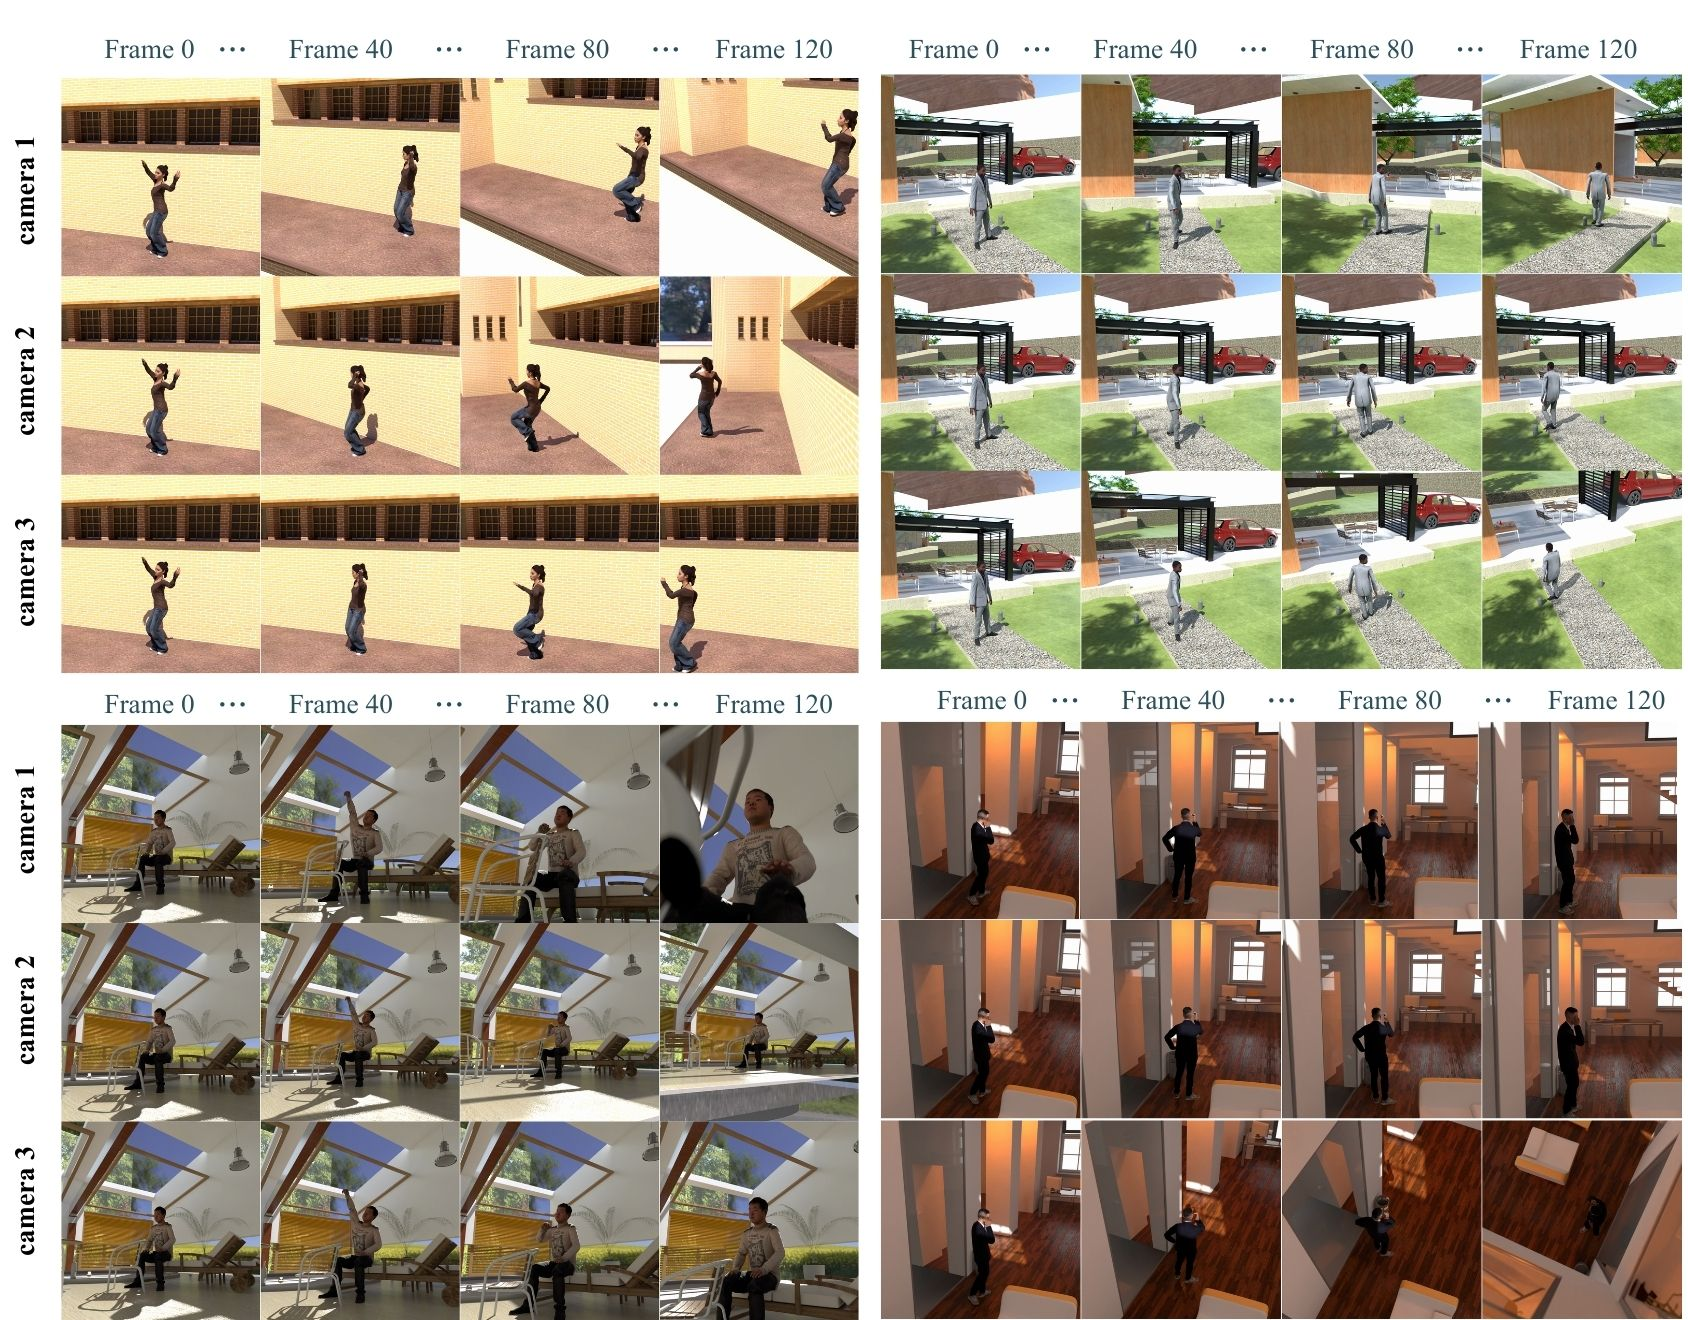
\includegraphics[width=\linewidth]{figures/src_files/data_demo.jpg}
    \caption{\textbf{Example of \nameDataset}.
   Multi-view, densely sampled sequences from the \nameDataset dataset. Each row shows frames from one camera trajectory, and each column samples different timesteps (0–120). The dataset provides diverse environments, human motions, and four camera paths per scene with full 120-frame temporal coverage.
    }
    \label{fig:visualexample}
\end{figure}

\begin{figure}[ht]
    \centering
    \vspace{-3mm}
    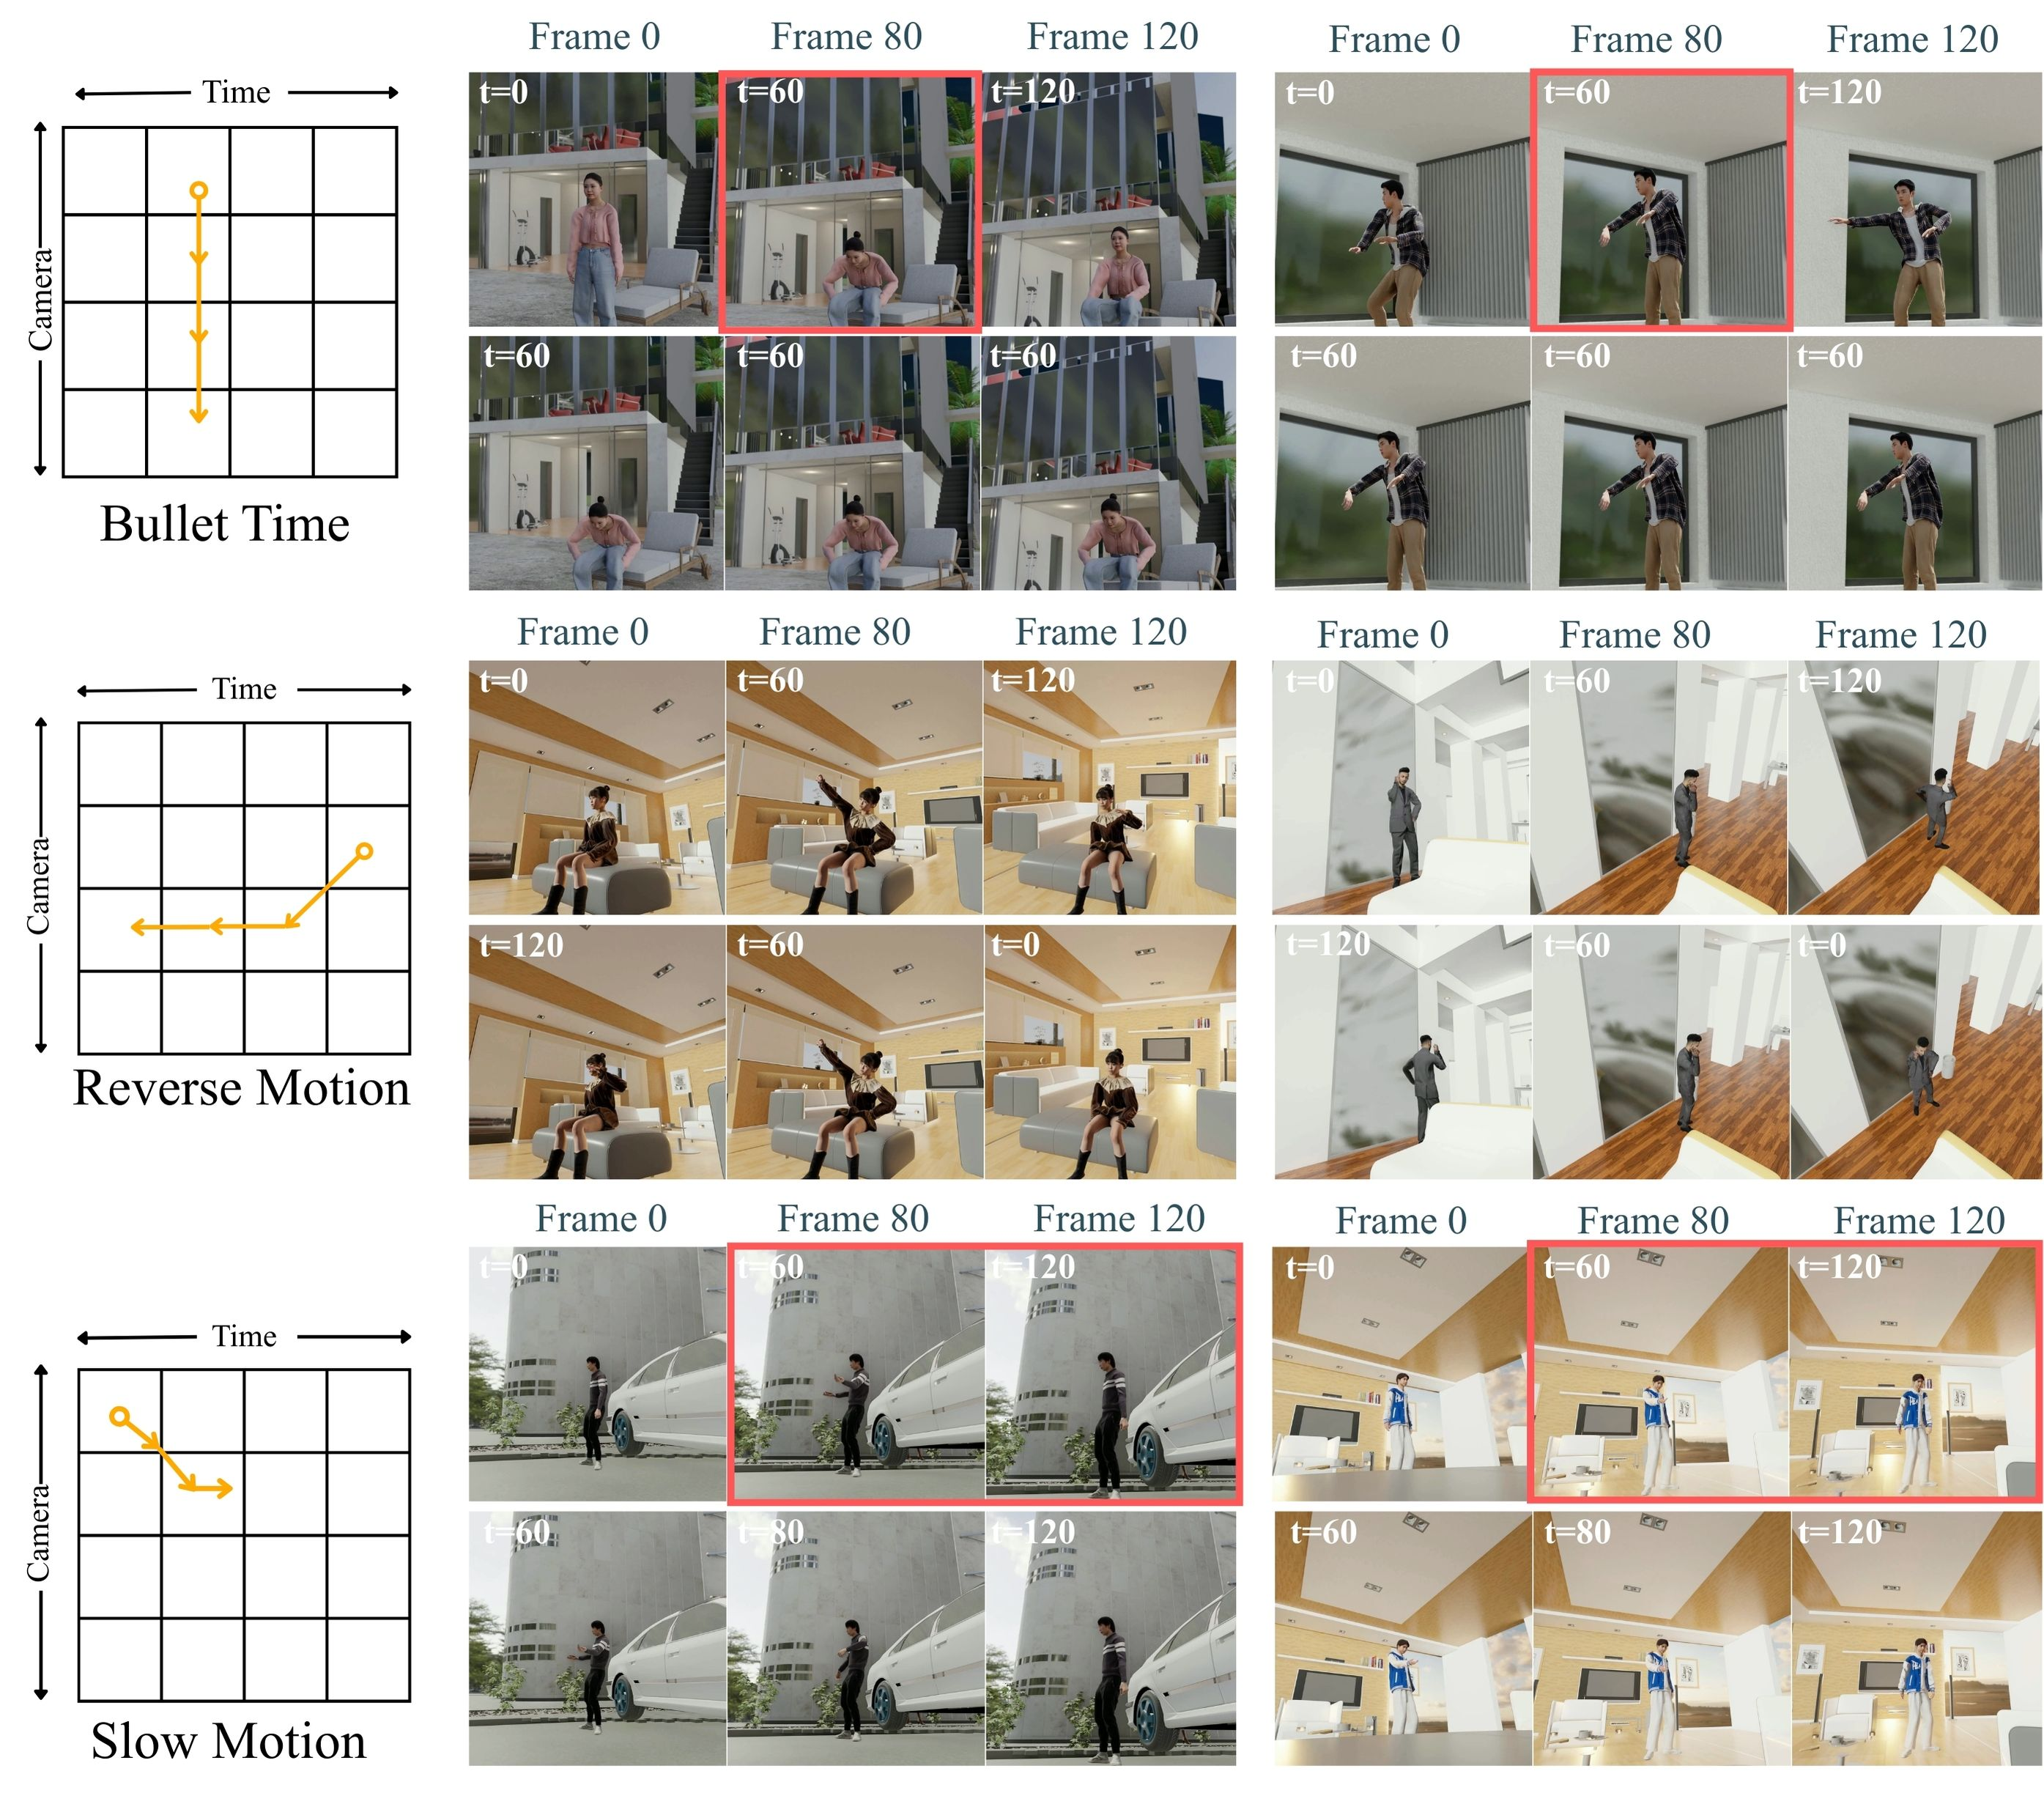
\includegraphics[width=\linewidth]{figures/src_files/sampling_example.jpg}
    
    \caption{
    \textbf{Sampling from \nameDataset.}
By sampling from the \nameDataset dataset, we can extract frames corresponding to arbitrary combinations of camera viewpoints and temporal positions, forming source-target pairs with rich camera and temporal control signals.
    }
    \label{fig:sampling}
\end{figure}

\begin{figure*}[ht]
    \centering
    \vspace{-3mm}
    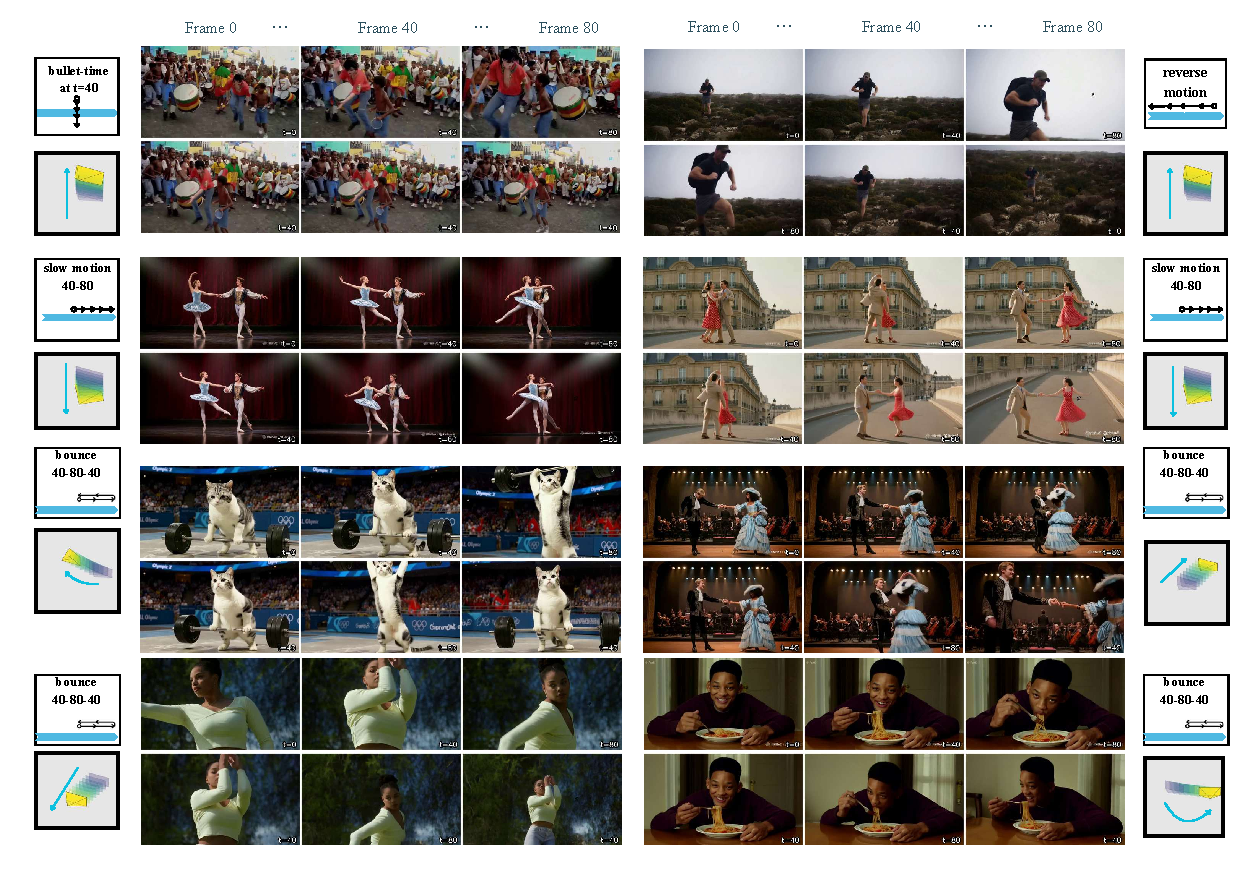
\includegraphics[width=\linewidth]{figures/more_results.pdf}
    \caption{
    \textbf{More Qualitative results.}
Our model provides fully disentangled control over camera motion and temporal dynamics. Each row illustrates a different combination of temporal control inputs (top-left icon) and camera trajectories. \nameMethod consistently produces coherent videos across a wide range of controls, including normal and reverse playback, bullet-time, slow motion, replay motion, and complex camera paths such as panning, tilting, zooming, and vertical motion.
    }
    \label{fig:more_quali}
\end{figure*}

